\documentclass{beamer}
\pdfstringdefDisableCommands{%
  \def\\{}%
  \def\texttt#1{<#1>}%
}
\beamertemplatenavigationsymbolsempty

\usepackage[italian]{babel}


% Footnote
\setbeamertemplate{footline}{\leavevmode%
  \begin{beamercolorbox}[wd=.33\paperwidth,left,ht=2.5ex,dp=1.5ex,rightskip=4pt plus 1pt, leftskip=4pt]{subsection in head/foot}
    Team 12
  \end{beamercolorbox}%
  \begin{beamercolorbox}[wd=.33\paperwidth,center,ht=2.5ex,dp=1.5ex]{section in head/foot}
  \end{beamercolorbox}%
  \begin{beamercolorbox}[wd=.34\paperwidth,ht=2.5ex,dp=1.5ex,leftskip=4pt plus 1pt,rightskip=4pt plus 1pt]{subsection in head/foot}
    \hfill\insertframenumber/\inserttotalframenumber
  \end{beamercolorbox}%
}


\title{Tweet analysis}
\author{
  \texorpdfstring{\parbox{45mm}{\centering\scriptsize Zaid Cheikh Ibrahim \\[-0.3em] {\tiny PO Operativo}}}{} \and 
  \texorpdfstring{\parbox{45mm}{\centering\scriptsize Tian Cheng Xia \\[-0.3em] {\tiny Scrum master}}}{}\\[1em]
  \texorpdfstring{\parbox{45mm}{\centering\scriptsize Qun Hao Henry Lee \\[-0.3em] {\tiny Developer}}}{} \and 
  \texorpdfstring{\parbox{45mm}{\centering\scriptsize Manuel Paris \\[-0.3em] {\tiny Developer}}}{}\\
}
\institute{
  Corso di Ingegneria del Software\\
  Alma Mater Studiorum $\cdot$ Università di Bologna  
}
\date{20 gennaio 2023}


\begin{document}

{
\setbeamertemplate{footline}{} 
\begin{frame}
  \titlepage
\end{frame}
}
\addtocounter{framenumber}{-1}


\begin{frame}
  \frametitle{Il prodotto}

  Client Twitter con le seguenti funzionalità:
  \begin{itemize}
    \item Ricerca e analisi di tweet
    \item Partita a scacchi contro gli utenti di Twitter
    \item Raccolta dell'esito dei giochi televisivi \textit{L'Eredità} e \textit{Reazione a Catena}
    \item Visualizzazione di una sintesi del Fantacitorio
  \end{itemize}
\end{frame}


\begin{frame}
  \frametitle{Raccolta e analisi di tweet}
    \begin{figure}[H]
      \centering
      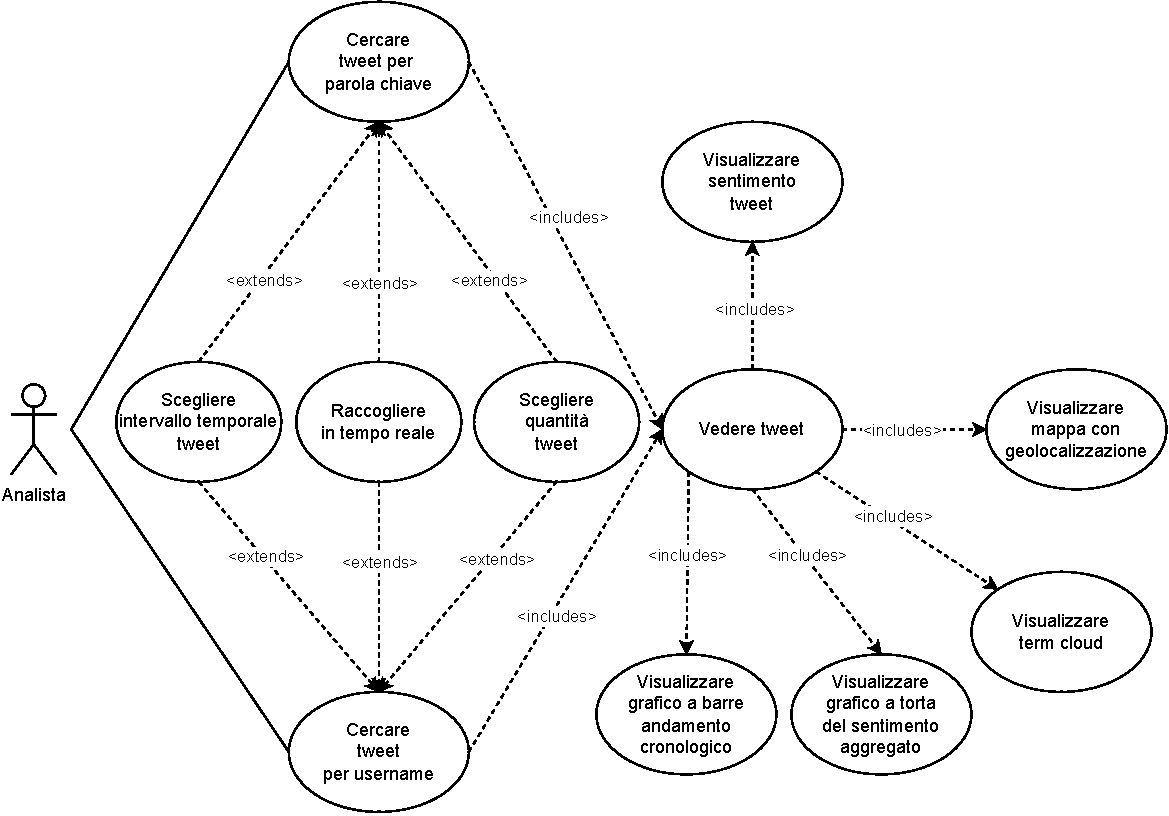
\includegraphics[scale=0.5]{../img/usecase/tweet.pdf}
  \end{figure}
\end{frame}


\begin{frame}
  \frametitle{Scacchi}
  \begin{figure}[H]
      \centering
      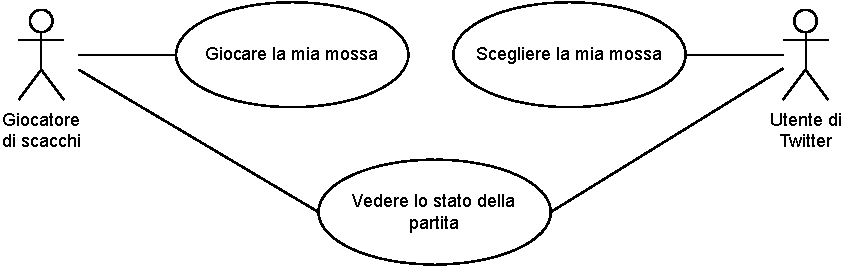
\includegraphics[scale=0.6]{../img/usecase/chess.pdf}
  \end{figure}
\end{frame}


\begin{frame}
  \frametitle{L'Eredità e Reazione a catena}
  \begin{figure}[H]
      \centering
      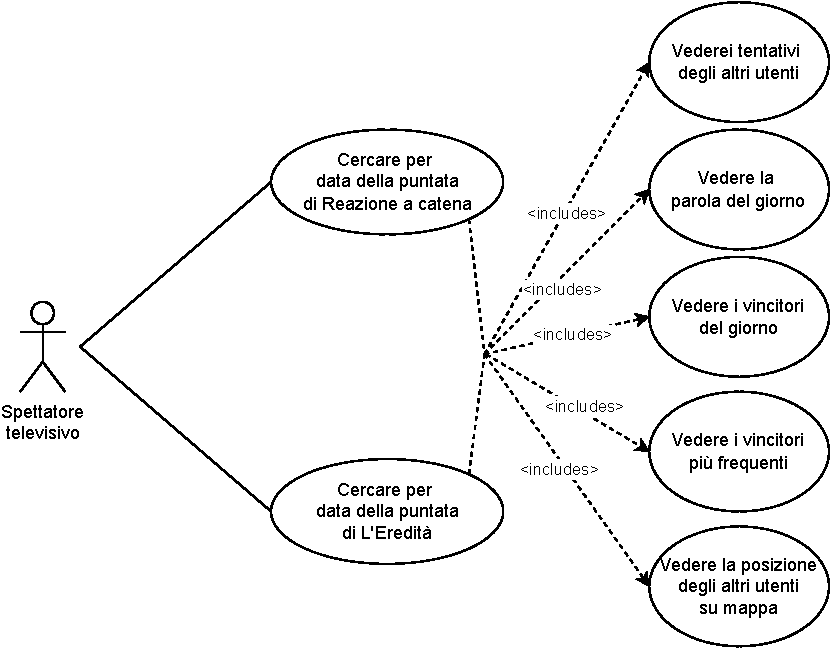
\includegraphics[scale=0.6]{../img/usecase/tvgames.pdf}
  \end{figure}
\end{frame}


\begin{frame}
  \frametitle{Fantacitorio}
  \begin{figure}[H]
      \centering
      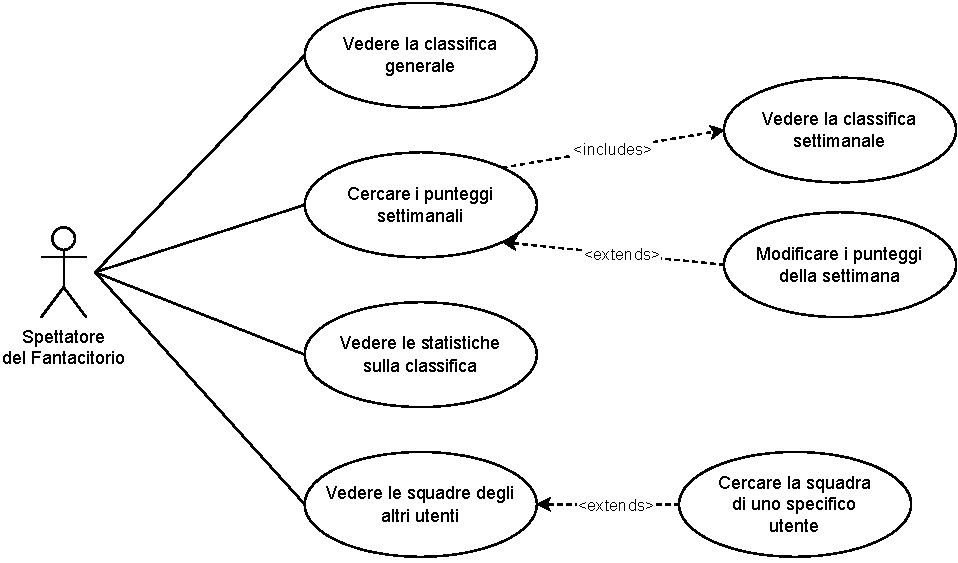
\includegraphics[scale=0.6]{../img/usecase/fantacitorio.pdf}
  \end{figure}
\end{frame}


\begin{frame}
  \frametitle{Sprint 1}
  \framesubtitle{Goal}

  \begin{itemize}
    \item Overview delle API di Twitter
    \item Realizzare i primi meccanismi di ricerca dei tweet
    \item Implementare le prime funzionalità per l'analisi dei dati
  \end{itemize}

\end{frame}

% \begin{frame}
%   \frametitle{Sprint 1}
%   \framesubtitle{Esito}
%   Sono state implementate le seguenti funzionalità:
%   \begin{itemize}
%     \item Ricerca per nome utente o hashtag e visualizzazione di tweet
%     \item Analisi del sentimento di un tweet
%   \end{itemize}
% \end{frame}

\begin{frame}
  \frametitle{Sprint 1}
  \framesubtitle{Esito}
  \begin{figure}[H]
      \centering
      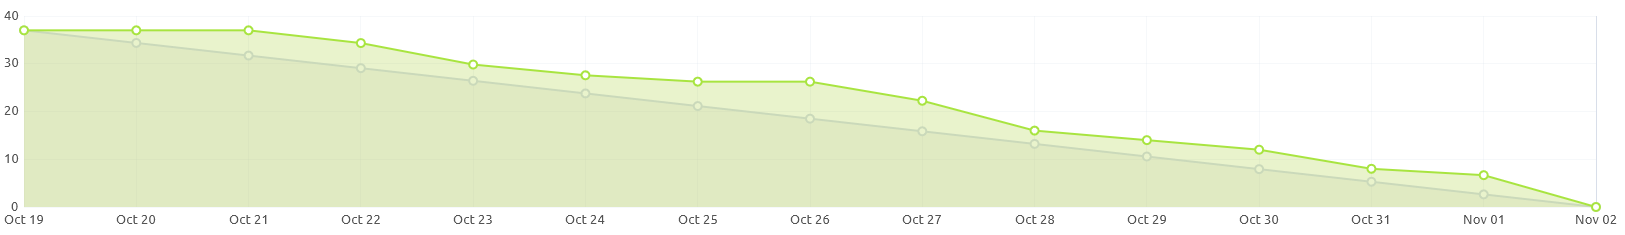
\includegraphics[width=\textwidth]{../img/sprint1/burndown.png}    
      \caption{Burndown sprint 1}
  \end{figure}
  \begin{figure}[H]
    \centering
    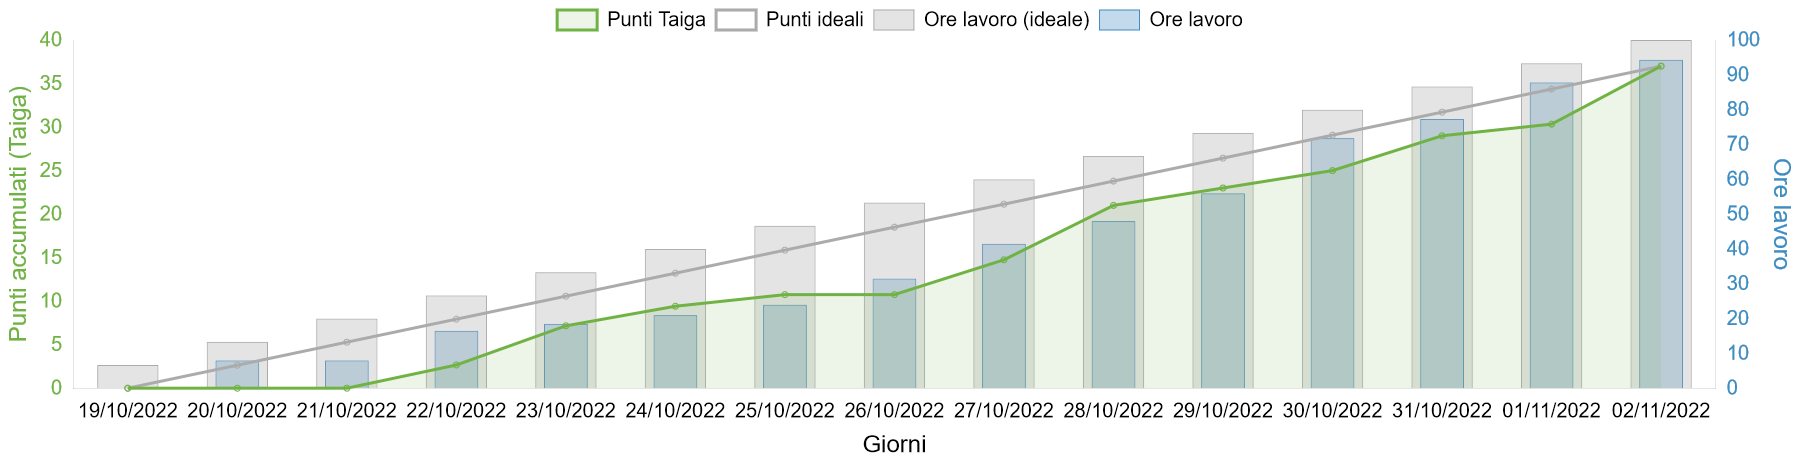
\includegraphics[width=\textwidth]{../img/sprint1/worktime.png}    
    \caption{Ore di lavoro sprint 1}
\end{figure}
\end{frame}


\begin{frame}
  \frametitle{Sprint 2}
  \framesubtitle{Goal}

  \begin{itemize}
    \item Implementare le richieste emerse allo sprint review precedente
    \item Concludere l'epica riguardante la visualizzazione e l'analisi dei tweet
  \end{itemize}
\end{frame}

% \begin{frame}
%   \frametitle{Sprint 2}
%   \framesubtitle{Esito}

%   Sono state implementate le seguenti funzionalità:
%   \begin{itemize}
%     \item Possibilità di selezionare il numero di tweet da raccogliere con una singola richiesta
%     \item Ricerca dei tweet per intervallo temporale
%     \item Ricerca dei tweet per parola chiave
%     \item Visualizzazione su mappa dei dati di geolocalizzazione dei tweet
%     \item Possibilità di raccogliere tweet in tempo reale
%   \end{itemize}
% \end{frame}

\begin{frame}
  \frametitle{Sprint 2}
  \framesubtitle{Esito}

  \begin{figure}
    \centering
    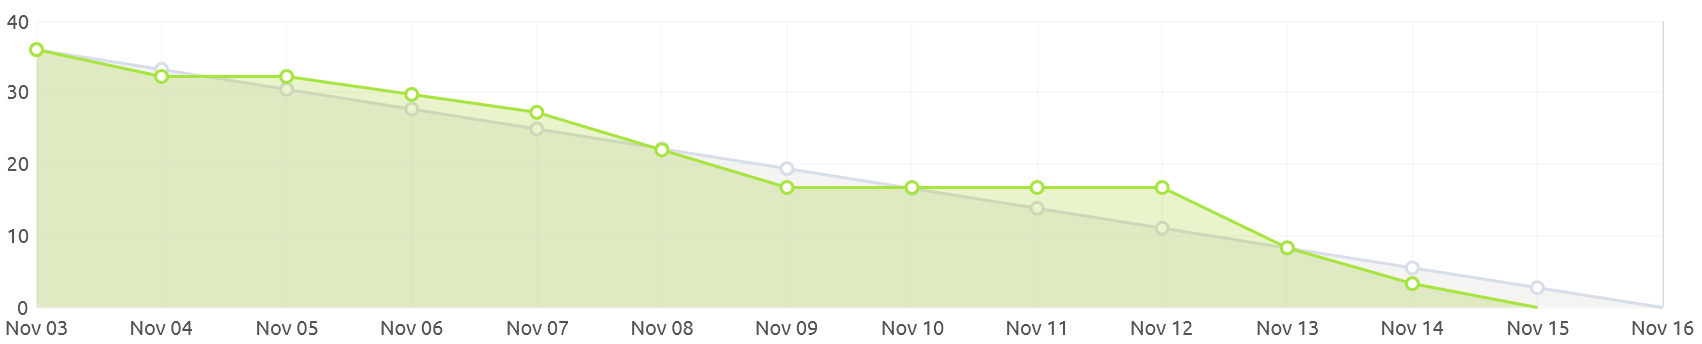
\includegraphics[width=\textwidth]{../img/sprint2/burndown.png}    
    \caption{Burndown sprint 2}
  \end{figure}
  \begin{figure}
    \centering
    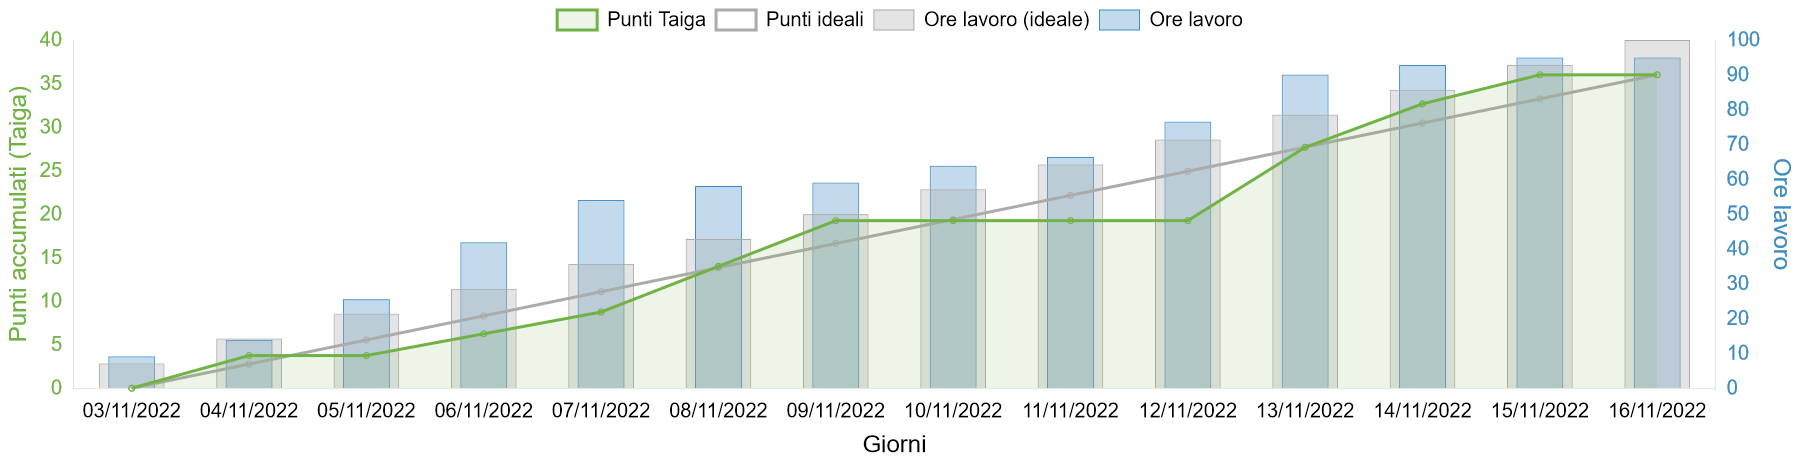
\includegraphics[width=\textwidth]{../img/sprint2/worktime.png}    
    \caption{Ore di lavoro sprint 2}
  \end{figure}
\end{frame}


\begin{frame}
  \frametitle{Sprint 3}
  \framesubtitle{Goal}

  \begin{itemize}
    \item Implementare le pagine per L'Eredità e Reazione a Catena
    \item Iniziare l'implementazione degli scacchi
  \end{itemize}
\end{frame}

% \begin{frame}
%   \frametitle{Sprint 3}
%   \framesubtitle{Esito}

%   Sono state implementate le seguenti funzionalità:
%   \begin{itemize}
%     \item Pagine per L'Eredità e Reazione a Catena
%     \begin{itemize}
%       \item  Selezionare la data di trasmissione
%       \item  Visualizzare i tentativi degli altri utenti
%       \item  Visualizzare la parola del giorno
%       \item  Visualizzare gli utenti che indovinano la parola
%       \item  Visualizzare la posizione degli utenti
%     \end{itemize}
%     \item Pagina per lo scacchi con la possibilità di giocare la propria mossa
%   \end{itemize}
% \end{frame}

\begin{frame}
  \frametitle{Sprint 3}
  \framesubtitle{Esito}

  \begin{figure}
    \centering
    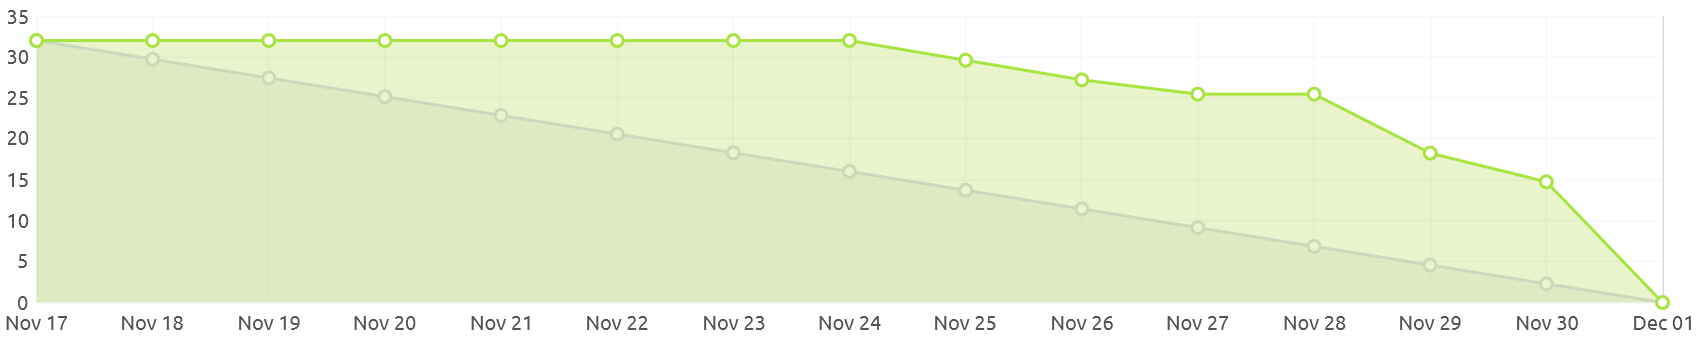
\includegraphics[width=\textwidth]{../img/sprint3/burndown.png}
    \caption{Burndown sprint 3}
  \end{figure}
  \begin{figure}
    \centering
    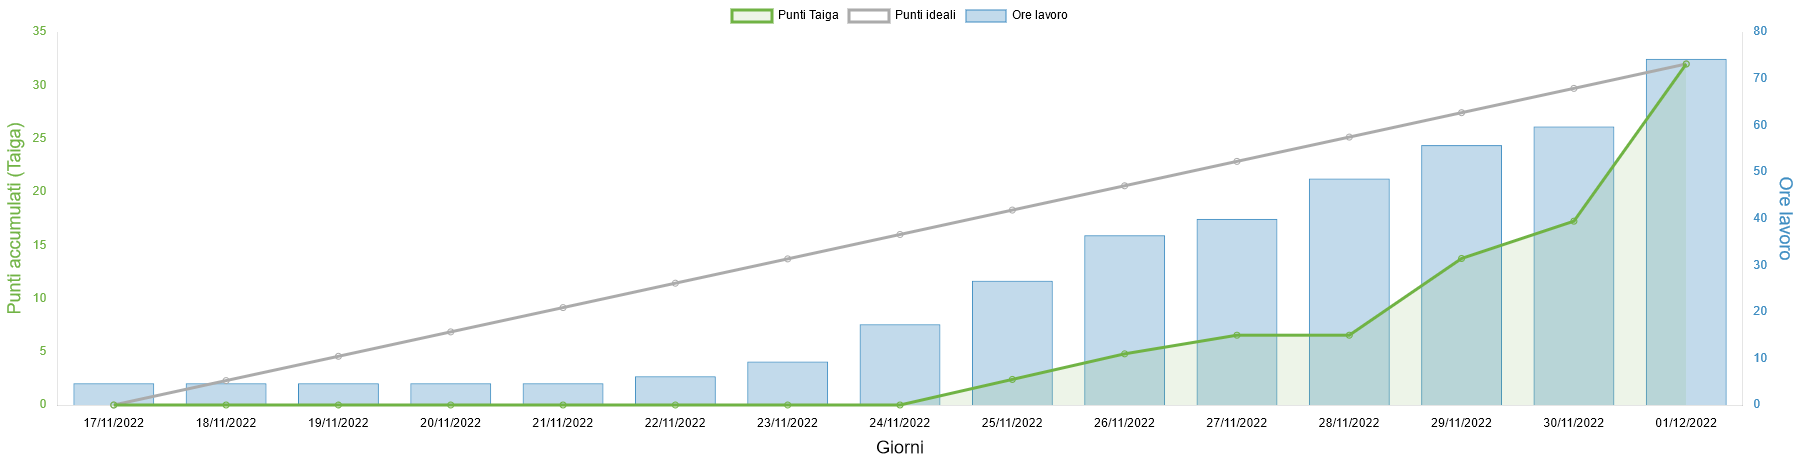
\includegraphics[width=\textwidth]{../img/sprint3/worktime.png}
    \caption{Ore di lavoro sprint 3}
  \end{figure}
\end{frame}


\begin{frame}
  \frametitle{Sprint 4}
  \framesubtitle{Goal}

  \begin{itemize}
    \item Implementare le funzionalità per il Fantacitorio
    \item Terminare gli scacchi
    \item Integrare i giochi televisivi con la richiesta del cliente
  \end{itemize}

\end{frame}

% \begin{frame}
%   \frametitle{Sprint 4}
%   \framesubtitle{Esito}

%   Sono state implementate le seguenti funzionalità:
%   \begin{itemize}
%       \item Per il Fantacitorio:
%       \begin{itemize}
%           \item Visualizzazione e modifica della classifica settimanale
%           \item Visualizzazione della classifica generale
%           \item Visualizzazione delle squadre degli altri giocatori
%           \item Ricerca della squadra di uno specifico utente
%           \item Statistiche sulla classifica
%       \end{itemize}
%       \item Per gli scacchi:
%       \begin{itemize}
%           \item Pubblicazione della scacchiera come tweet
%           \item Raccolta e selezione della mossa dell'avversario a maggioranza
%       \end{itemize}
%       \item Per i giochi televisivi:
%       \begin{itemize}
%           \item Visualizzazione dei più vincenti in un periodo di tempo
%       \end{itemize}
%   \end{itemize}
% \end{frame}

\begin{frame}
  \frametitle{Sprint 4}
  \framesubtitle{Esito}

  \begin{figure}
    \centering
    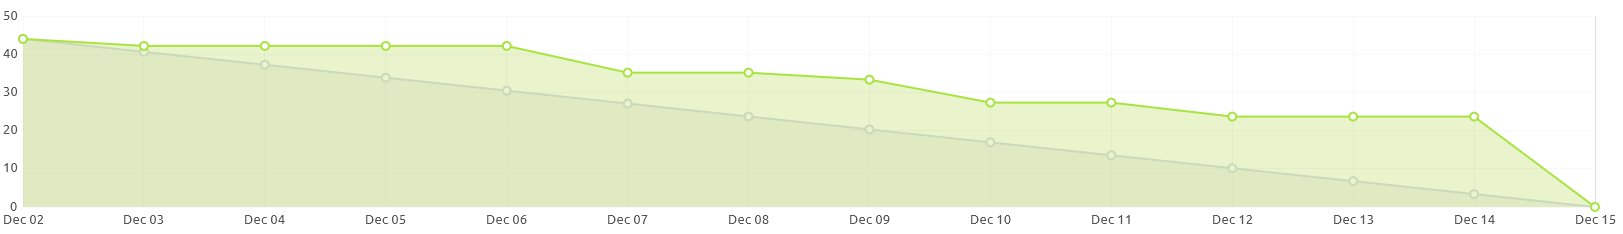
\includegraphics[width=\textwidth]{../img/sprint4/burndown.png}
    \caption{Burndown sprint 4}
  \end{figure}
  \begin{figure}
    \centering
    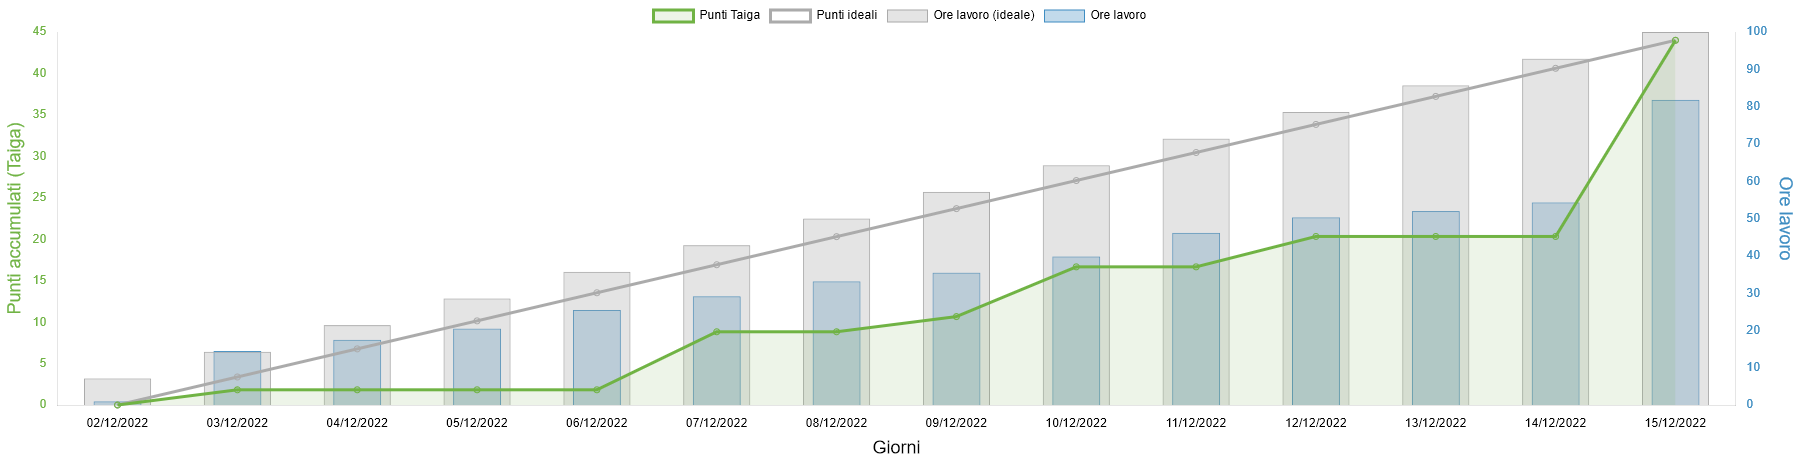
\includegraphics[width=\textwidth]{../img/sprint4/worktime.png}
    \caption{Ore di lavoro sprint 4}
  \end{figure}
\end{frame}


\begin{frame}
  \frametitle{Sonarqube}
  \begin{figure}[H]
      \centering
      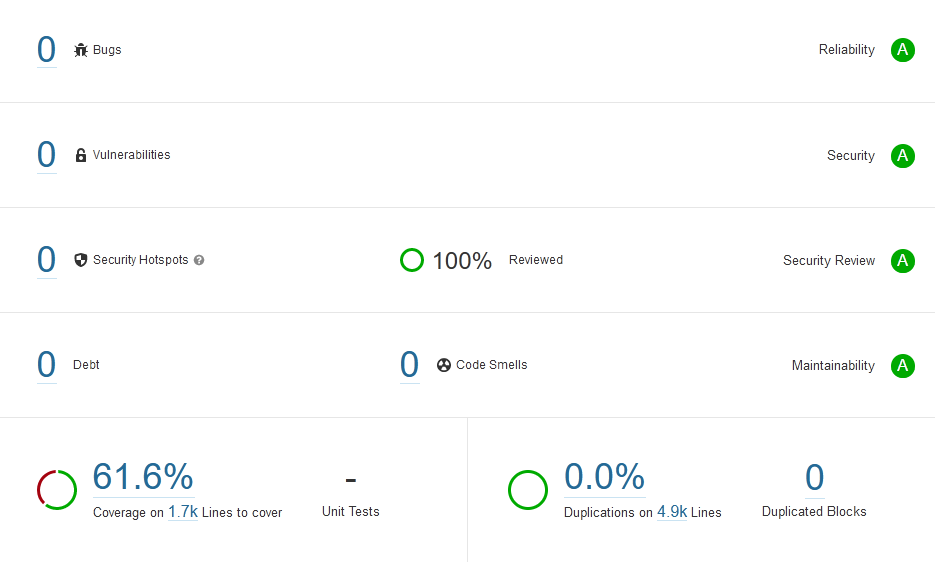
\includegraphics[scale=0.42]{../img/sprint4/sonarqube.png}
  \end{figure}
\end{frame}


\begin{frame}
  \frametitle{Flusso di lavoro}
  \begin{figure}[H]
      \centering
      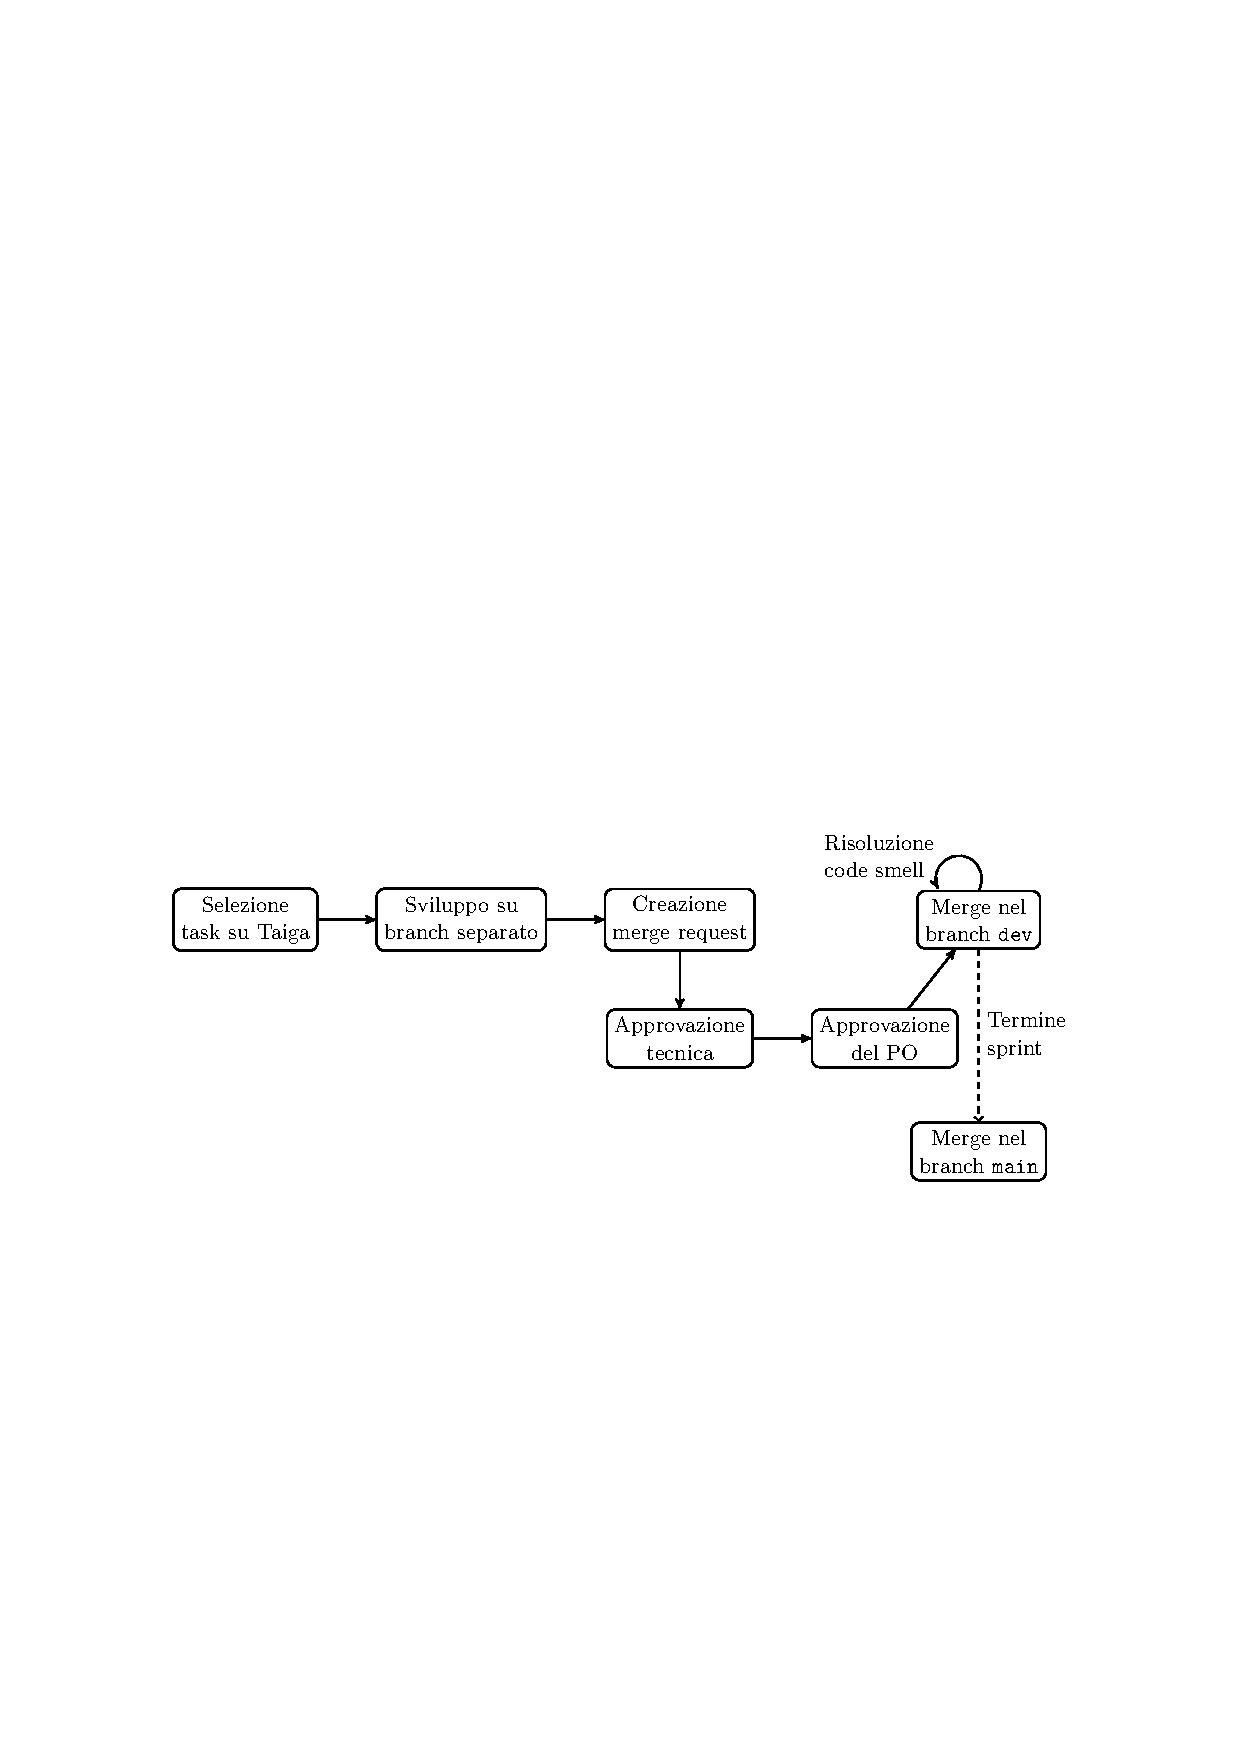
\includegraphics[scale=0.65]{../img/slides/workflow.pdf}
  \end{figure}
\end{frame}


\begin{frame}
  \frametitle{Deployment}
  \begin{figure}[H]
      \centering
      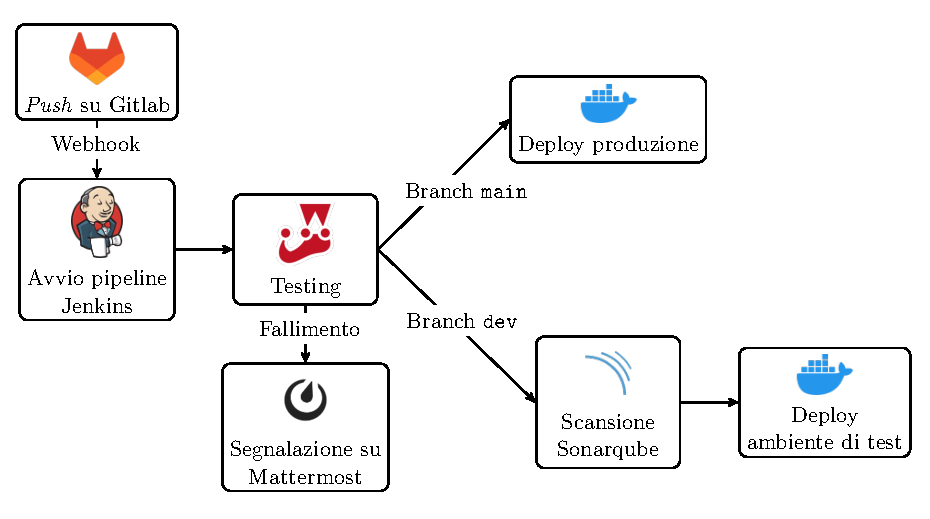
\includegraphics[scale=0.65]{../img/slides/deployment.pdf}
  \end{figure}
\end{frame}


\end{document}